\documentclass[11pt,openany]{article}

\usepackage{mathtools, commath}
% Packages for formatting
\usepackage[margin=1in]{geometry}
\usepackage{fancyhdr}
\usepackage{enumerate}
\usepackage{graphicx}
\usepackage{kotex}
\usepackage{arydshln} % Include this package
\usepackage{bbding}
\usepackage{amsmath}
\usepackage{amsthm}
\usepackage[dvipsnames,table]{xcolor}
\usepackage{amssymb, amsfonts}
\usepackage{wasysym}
\usepackage{footnote}
\usepackage{tablefootnote}
\usepackage{arydshln} % Include this package
% Fonts
\usepackage[T1]{fontenc}
\usepackage[utf8]{inputenc}
\usepackage{newpxtext,newpxmath}
\usepackage{sectsty}

% Define colors
\definecolor{TealBlue1}{HTML}{0077c2}
\definecolor{TealBlue2}{HTML}{00a5e6}
\definecolor{TealBlue3}{HTML}{b3e0ff}
\definecolor{TealBlue4}{HTML}{00293c}
\definecolor{TealBlue5}{HTML}{e6f7ff}

\definecolor{thmcolor}{RGB}{231, 76, 60}
\definecolor{defcolor}{RGB}{52, 152, 219}
\definecolor{lemcolor}{RGB}{155, 89, 182}
\definecolor{corcolor}{RGB}{46, 204, 113}
\definecolor{procolor}{RGB}{241, 196, 15}

\usepackage{color,soul}
\usepackage{soul}
\newcommand{\mathcolorbox}[2]{\colorbox{#1}{$\displaystyle #2$}}
\usepackage{cancel}
\newcommand\crossout[3][black]{\renewcommand\CancelColor{\color{#1}}\cancelto{#2}{#3}}
\newcommand\ncrossout[2][black]{\renewcommand\CancelColor{\color{#1}}\cancel{#2}}

\usepackage{hyperref}
\usepackage{booktabs}

% Chapter formatting
\definecolor{titleTealBlue}{RGB}{0,53,128}
\usepackage{titlesec}
\titleformat{\section}
{\normalfont\sffamily\Large\bfseries\color{titleTealBlue!100!gray}}{\thesection}{1em}{}
\titleformat{\subsection}
{\normalfont\sffamily\large\bfseries\color{titleTealBlue!50!gray}}{\thesubsection}{1em}{}

%Tcolorbox
\usepackage[most]{tcolorbox}
\usepackage{multirow}
\usepackage{multicol}

\usepackage[linesnumbered,ruled]{algorithm2e}
\usepackage{algpseudocode}
\usepackage{setspace}
\SetKwComment{Comment}{/* }{ */}
\SetKwProg{Fn}{Function}{:}{end}
\SetKw{End}{end}
\SetKw{DownTo}{downto}

% Define a new environment for algorithms without line numbers
\newenvironment{algorithm2}[1][]{
	% Save the current state of the algorithm counter
	\newcounter{tempCounter}
	\setcounter{tempCounter}{\value{algocf}}
	% redefine the algorithm numbering (remove prefix)
	\renewcommand{\thealgocf}{}
	\begin{algorithm}
	}{
	\end{algorithm}
	% Restore the algorithm counter state
	\setcounter{algocf}{\value{tempCounter}}
}

\usepackage{adjustbox}
% Header and footer formatting
\pagestyle{fancy}
\fancyhead{}
\fancyhf{}
\rhead{\textcolor{TealBlue2}{\large\textbf{기대수(기초부터 대학원 수학까지 시리즈) 3기}}}%\rule{3cm}{0.4pt}}
\lhead{\textcolor{TealBlue2}{\large\textbf{수학의 즐거움, Enjoying Math}}}
% Define footer
%\newcommand{\footer}[1]{
%\begin{flushright}
%	\vspace{2em}
%	\includegraphics[width=2.5cm]{school_logo.jpg} \\
%	\vspace{1em}
%	\textcolor{TealBlue2}{\small\textbf{#1}}
%\end{flushright}
%}
%\rfoot{\large Department of Information Security, Cryptogrphy and Mathematics, Kookmin Uni.\includegraphics[height=1.5cm]{school_logo.jpg}}
\fancyfoot{}
\fancyfoot[C]{-\thepage-}

\usepackage{tcolorbox}
\tcbset{colback=white, arc=5pt}

\definecolor{axiomcolor}{HTML}{a88bfa}
\definecolor{defcolor}{RGB}{52, 152, 219}
\definecolor{procolor}{RGB}{241, 196, 15}
\definecolor{thmcolor}{RGB}{231, 76, 60}
\definecolor{lemcolor}{RGB}{155, 89, 182}
\definecolor{corcolor}{RGB}{46, 204, 113}
\definecolor{execolor}{RGB}{90, 128, 127}

% Define a new command for the custom tcolorbox
\newcommand{\axiombox}[2][]{%
	\begin{tcolorbox}[colframe=axiomcolor, title={\color{white}\bfseries #1}]
		#2
	\end{tcolorbox}
}

\newcommand{\defbox}[2][]{%
	\begin{tcolorbox}[colframe=defcolor, title={\color{white}\bfseries #1}]
		#2
	\end{tcolorbox}
}

\newcommand{\lembox}[2][]{%
	\begin{tcolorbox}[colframe=lemcolor, title={\color{white}\bfseries #1}]
		#2
	\end{tcolorbox}
}

\newcommand{\probox}[2][]{%
	\begin{tcolorbox}[colframe=procolor, title={\color{white}\bfseries #1}]
		#2
	\end{tcolorbox}
}

\newcommand{\thmbox}[2][]{%
	\begin{tcolorbox}[colframe=thmcolor, title={\color{white}\bfseries #1}]
		#2
	\end{tcolorbox}
}

\newcommand{\corbox}[2][]{%
	\begin{tcolorbox}[colframe=corcolor, title={\color{white}\bfseries #1}]
		#2
	\end{tcolorbox}
}



\usepackage{amsthm}

% Define custom theorem styles
\newtheoremstyle{dotless} % Name of the style
{3pt} % Space above
{3pt} % Space below
{\itshape} % Body font
{} % Indent amount
{\bfseries} % Theorem head font
{} % Punctuation after theorem head
{2.5mm} % Space after theorem head
{} % Theorem head spec

\newtheoremstyle{definitionstyle} % Name of the style
{3pt} % Space above
{3pt} % Space below
{} % Body font
{} % Indent amount
{\bfseries} % Theorem head font
{.} % Punctuation after theorem head
{2.5mm} % Space after theorem head
{} % Theorem head spec

% Applying custom styles
\theoremstyle{dotless}
\newtheorem{theorem}{Theorem} % Theorem environment with section-wise numbering
\newtheorem{proposition}[theorem]{Proposition} % Theorem environment with section-wise numbering
\newtheorem{lemma}[theorem]{Lemma} % Lemma shares the counter with theorem
\newtheorem{corollary}[theorem]{Corollary} % Corollary shares the counter with theorem

\theoremstyle{definitionstyle}
\newtheorem*{observation}{\textcolor{Magenta}{Observation}}
\newtheorem{definition}{Definition} % Definition shares the counter with theorem
\newtheorem{example}{Example} % Example shares the counter with theorem
\newtheorem{exercise}{Exercise} % Example shares the counter with theorem
\newtheorem{remark}{Remark} % Remark shares the counter with theorem
\newtheorem*{note}{Note}

\newtheorem*{definition*}{Definition} % Definition shares the counter with theorem
\newtheorem*{example*}{Example} % Example shares the counter with theorem
\newtheorem*{exercise*}{\textcolor{violet}{Exercise}} % Example shares the counter with theorem
\newtheorem*{remark*}{Remark} % Remark shares the counter with theorem


\usepackage{tikz}
\usepackage{tikz-cd}
\usepackage{tikz-3dplot}
\usepackage{pgfplots}
\pgfplotsset{compat=newest} % Adjust to your version of pgfplots
\def\Circlearrowleft{\ensuremath{%
		\rotatebox[origin=c]{180}{$\circlearrowleft$}}}
\def\Circlearrowright{\ensuremath{%
		\rotatebox[origin=c]{180}{$\circlearrowright$}}}
\def\CircleArrowleft{\ensuremath{%
		\reflectbox{\rotatebox[origin=c]{180}{$\circlearrowleft$}}}}
\def\CircleArrowright{\ensuremath{%
		\reflectbox{\rotatebox[origin=c]{180}{$\circlearrowright$}}}}
\usetikzlibrary{
	3d, % For 3D drawing
	angles,
	arrows,
	arrows.meta,
	backgrounds,
	bending,
	calc,
	decorations.pathmorphing,
	decorations.pathreplacing,
	decorations.markings,
	fit,
	matrix,
	patterns,
	patterns.meta,
	positioning,
	quotes,
	shadows,
	shapes,
	shapes.geometric,
	tikzmark
}
\tikzset{
	% single mid‐path arrow
	mid arrow/.style={
		decoration={
			markings,
			mark=at position 0.5 with {\arrow{Stealth[scale=1.2]}}
		},
		postaction={decorate},
	},
	% style for field arrows
	field arrow/.style={
		-{Stealth[scale=1.0]},
		thick,
		blue!70!black,
	},
}
\newcommand{\ie}{\textnormal{i.e.}}
\newcommand{\rsa}{\mathsf{RSA}}
\newcommand{\rsacrt}{\mathsf{RSA}\textendash\mathsf{CRT}}
\newcommand{\inv}[1]{#1^{-1}}

%New Command
%\newcommand{\set}[1]{\left\{#1\right\}}
\newcommand{\N}{\mathbb{N}}
\newcommand{\Z}{\mathbb{Z}}
\newcommand{\Q}{\mathbb{Q}}
\newcommand{\R}{\mathbb{R}}
\newcommand{\cR}{\mathcal{R}}
\newcommand{\C}{\mathbb{C}}
\newcommand{\F}{\mathbb{F}}
\newcommand{\nbhd}{\mathcal{N}}
\newcommand{\Log}{\operatorname{Log}}
\newcommand{\Arg}{\operatorname{Arg}}
\newcommand{\pv}{\operatorname{P.V.}}

\newcommand{\of}[1]{\left( #1 \right)} 
%\newcommand{\abs}[1]{\left\lvert #1 \right\rvert}
%\newcommand{\norm}[1]{\left\| #1 \right\|}

\newcommand{\sol}{\textcolor{magenta}{\bf Sol}}
\newcommand{\conjugate}[1]{\overline{#1}}

\newcommand{\res}{\operatorname{res}}
\DeclareMathOperator*{\Res}{\operatorname{Res}}

%\renewcommand{\Re}{\operatorname{Re}}
%\renewcommand{\Im}{\operatorname{Im}}

\newcommand{\cyclic}[1]{\langle #1 \rangle}
\newcommand{\uniform}{\overset{\$}{\leftarrow}}
\newcommand{\xmark}{\textcolor{red}{\XSolidBrush}}
\newcommand{\vmark}{\textcolor{green!75!black}{\CheckmarkBold}}

\newcommand{\gen}[1]{\langle #1 \rangle}
\newcommand{\Gen}[1]{\left\langle #1 \right\rangle}

\newcommand{\img}[1]{\text{Img}(#1)}
\newcommand{\Img}[1]{\text{Img}\left(#1\right)}
\newcommand{\preimg}[1]{\text{Img}^{-1}(#1)}
\newcommand{\Preimg}[1]{\text{Img}^{-1}\left(#1\right)}

\newcommand{\relation}{\mathrel{\mathcal{R}}}
\newcommand{\injection}{\rightarrowtail}
\newcommand{\surjection}{\twoheadrightarrow}
\newcommand{\id}{\textnormal{id}}

\newcommand{\eqclass}[1]{\left[#1\right]}

% Define custom colors for O and X
\newcommand{\yes}{\textcolor{blue}{\bf \fullmoon}}
\newcommand{\no}{\textcolor{red}{\bf \texttimes}}

\DeclarePairedDelimiter\ceil{\lceil}{\rceil}
\DeclarePairedDelimiter\floor{\lfloor}{\rfloor}
%\renewcommand{\floor}[#1]{\lfloor #1\rfloor}
%\newcommand{\Floor}[#1]{\left\lfloor #1\right\rfloor}
%\newcommand{\ceil}[#1]{\lceil #1\rceil}
%\newcommand{\Ceil}[#1]{\left\lceil #1\right\rceil}

\newcommand{\topology}{\mathscr{T}}
\newcommand{\sequence}[1]{\langle #1\rangle}
\renewcommand{\vec}[1]{\mathbf{#1}}
\renewcommand{\Re}{\operatorname*{Re}}
\renewcommand{\Im}{\operatorname*{Im}}
\setstretch{1.25}

%\usepackage{background}
%\backgroundsetup{
%	scale=3,
%	color=gray!20,
%	opacity=0.3,
%	angle=45,
%	contents={\Huge \sffamily Ji, Yong-hyeon}
%}
\begin{document}
\pagenumbering{arabic}
\begin{center}
	\huge\textbf{Abstract Algebra I}\\
	\vspace{0.5em}
	\large{Ji, Yong-hyeon}\\
%	\large{\ttfamily \url{https://github.com/Hacker-Code-J}}\\
	\vspace{0.5em}
	\normalsize{\today}\\
\end{center}

\noindent 
We cover the following topics in this note.
\begin{itemize}
	\item Cyclic Group
	\item TBA
\end{itemize}
\hrule\vspace{12pt}
%\tableofcontents
\newpage

%We develop the concept of cyclic groups and establish their complete classification.

\begin{note}
Let \( (G, \ast) \) be a group with identity element \( e \). Recall that the axioms of a group require:
\begin{enumerate}[(G1)]
	\item[(G0)] $\forall\, x, y \in G,  x \ast y\in G$;
	\item $\forall\, x, y, z \in G,\;  (x \ast y) \ast z = x \ast (y\ast z)$;
	\item $\exists\, e \in G,\; \text{s.t.}\; \forall\, x \in G,\; e \cdot x = x \cdot e = x$;
	\item $\forall\, x \in G,\; \exists\, x^{-1} \in G\; \text{s.t.}\; x \cdot x^{-1} = x^{-1} \cdot x = e$.
\end{enumerate}
Consider \((\mathbb{Z},+)\) as the additive group of integers. For \( a \in G \) and \( n \in \mathbb{Z} \), the notation
\[
a^n \coloneqq
\begin{cases}
	\underbrace{a \ast a \ast \cdots \ast a}_{n \text{ times}} &: n > 0, \\
	e &: n = 0, \\
	(a^{-1})^{-n}&: n < 0,
\end{cases}
\]
defines the \( n \)-th power of \( a \).
\end{note}
\defbox[Cyclic Group]{\begin{definition*}
	A group $G$ is said to be \textbf{cyclic} if and only if \[
	\exists\, a \in G \;\text{such that}\; \Bigl[\, \forall\, g \in G,\; \exists\, n \in \mathbb{Z} \text{ with } g = a^n \Bigr].
	\] The element \( a \) is called a \textbf{generator} of \( G \).
\end{definition*}}

\thmbox[The Classification for Cyclic Groups]{\begin{theorem*}
Let \(G\) be a cyclic group. Then
\[
G \simeq
\begin{cases}
	\mathbb{Z} & \text{if } G \text{ is infinite,} \\
	\mathbb{Z}/n\mathbb{Z} & \text{if } G \text{ is finite of order } n.
\end{cases}
\] In other words, Every cyclic group $G$ is isomorphic to either $\mathbb{Z}$ or $\mathbb{Z}/n\mathbb{Z}$ for some $n \in \mathbb{N}$.	
\end{theorem*}}
\begin{proof}
	Let \( G \) be a cyclic group and let \( a \in G \) be a generator. Define the mapping
	\[
	\varphi : (\mathbb{Z}, +) \to (G, \ast), \quad \varphi(n) = a^n.
	\]
	We now verify several properties of \(\varphi\).
\end{proof}

\newpage


%
%#### 2.3.1 \(\varphi\) is a Homomorphism
%
%For all \( m, n \in \mathbb{Z} \), we have:
%\[
%\varphi(m+n) = a^{m+n} = a^m \cdot a^n = \varphi(m) \cdot \varphi(n).
%\]
%Thus, \(\varphi\) is a group homomorphism.
%
%#### 2.3.2 Surjectivity of \(\varphi\)
%
%Since \( G = \langle a \rangle \), by definition every \( g \in G \) may be expressed as \( g = a^n \) for some \( n \in \mathbb{Z} \). Hence, \(\varphi\) is surjective.
%
%#### 2.3.3 Kernel of \(\varphi\)
%
%Define the kernel of \(\varphi\) by
%\[
%\ker(\varphi) \coloneqq \{\, n \in \mathbb{Z} \mid a^n = e \,\}.
%\]
%Since \(\ker(\varphi)\) is a subgroup of \(\mathbb{Z}\), and every subgroup of \(\mathbb{Z}\) is of the form
%\[
%d\mathbb{Z} = \{\, d k \mid k \in \mathbb{Z} \,\},
%\]
%for some \( d \in \mathbb{Z}_{\ge 0} \), we have
%\[
%\ker(\varphi) = d\mathbb{Z}.
%\]
%Two cases arise:
%
%- **Case 1: \( d = 0 \).**  
%In this case, 
%\[
%\ker(\varphi) = \{0\},
%\]
%and by the First Isomorphism Theorem, we obtain:
%\[
%G \cong \mathbb{Z}/\{0\} \cong \mathbb{Z}.
%\]
%Thus, \( G \) is infinite.
%
%- **Case 2: \( d > 0 \).**  
%There exists a unique minimal positive integer \( d \) (namely, the order of \( a \)) such that
%\[
%a^d = e.
%\]
%Then,
%\[
%\ker(\varphi) = d\mathbb{Z},
%\]
%and the First Isomorphism Theorem yields:
%\[
%G \cong \mathbb{Z}/d\mathbb{Z}.
%\]
%In this case, \( G \) is finite with \(|G| = d\).
%
%#### 2.3.4 Statement of the Classification Theorem
%
%\[
%\boxed{
%	\textbf{Theorem.} \quad 
%}
%\]
%
%### 2.4 Discussion
%
%The above results establish that the algebraic structure of cyclic groups is entirely determined by the order of a generator. In summary:
%
%- A group \( G \) is cyclic if and only if
%\[
%\exists\, a \in G \; \forall\, g \in G,\; \exists\, n \in \mathbb{Z} \text{ with } g = a^n.
%\]
%- The mapping \(\varphi : \mathbb{Z} \to G\) defined by \( n \mapsto a^n \) is a surjective group homomorphism.
%- The kernel of \(\varphi\) is of the form \( d\mathbb{Z} \) for some \( d \ge 0 \); thus, \( G \cong \mathbb{Z}/d\mathbb{Z} \).
%- In the case \( d = 0 \), the group is infinite and isomorphic to \( \mathbb{Z} \); when \( d > 0 \), it is finite of order \( d \) and isomorphic to \( \mathbb{Z}/d\mathbb{Z} \).
%
%This classification underscores the fundamental simplicity and ubiquity of cyclic groups in group theory, serving as a cornerstone for further studies in algebra.
%
%---
%
%This exposition is designed to meet the standards of rigorous mathematical literature suitable for publication at the graduate level.



%### 1. Definition of a Cyclic Group

\[
\textbf{Definition.} \quad G \text{ is called \emph{cyclic} } \iff \exists\, a \in G \text{ such that } G = \langle a \rangle \coloneqq \{\, a^n \mid n \in \mathbb{Z} \,\}.
\]

In symbolic logic, this may be written as:
\[
\exists\, a \in G \;\; \forall\, g \in G,\; \exists\, n \in \mathbb{Z} \text{ such that } g = a^n.
\]

Here, the element \(a\) is called a \emph{generator} of \(G\). The notation \(a^n\) is understood in the group-theoretic sense, where for \(n \ge 0\), 
\[
a^n = \underbrace{a \cdot a \cdots a}_{n\text{ factors}},
\]
and for \(n < 0\), 
\[
a^n = (a^{-1})^{-n}.
\]

%---

%### 2. Classification of Cyclic Groups

The structure of cyclic groups is completely determined by the order of any generator. Let \( a \in G \) be a generator of the cyclic group \(G\). Consider the homomorphism 
\[
\varphi : (\mathbb{Z}, +) \to (G, \cdot) \quad \text{defined by} \quad \varphi(n) = a^n.
\]
Since \( G \) is cyclic, \(\varphi\) is surjective. The kernel of \(\varphi\) is given by
\[
\ker(\varphi) = \{\, n \in \mathbb{Z} \mid a^n = e \,\},
\]
where \(e\) denotes the identity element in \(G\).

We now distinguish two cases:

1. **Infinite Case:**  
If no nonzero \( n \in \mathbb{Z} \) satisfies \( a^n = e \), then
\[
\ker(\varphi) = \{0\}.
\]
By the First Isomorphism Theorem, 
\[
G \cong \mathbb{Z}.
\]

2. **Finite Case:**  
If there exists a least positive integer \( n_0 \) such that
\[
a^{n_0} = e,
\]
then 
\[
\ker(\varphi) = n_0 \mathbb{Z} \coloneqq \{\, n_0 k \mid k \in \mathbb{Z} \,\}.
\]
Again by the First Isomorphism Theorem,
\[
G \cong \mathbb{Z}/n_0 \mathbb{Z}.
\]
In this context, we say that \(G\) is of \emph{finite order} \(n_0\).

Thus, we have the following classification theorem:

\[
\boxed{
	\text{Every cyclic group } G \text{ is isomorphic to either } \mathbb{Z} \text{ (if } |G| = \infty \text{) or } \mathbb{Z}/n\mathbb{Z} \text{ for some } n \in \mathbb{N} \text{ (if } |G| = n < \infty \text{).}
}
\]

---

%### 3. Summary of the Logical Structure

- **Existence of Generator:**  
\(\exists\, a \in G\) such that \(\forall\, g \in G\), \(\exists\, n \in \mathbb{Z}\) with \(g = a^n\).

- **Homomorphism Construction:**  
Define \(\varphi: \mathbb{Z} \to G\) by \(\varphi(n) = a^n\). This map is a group homomorphism with image \(G\).

- **Kernel Analysis:**
- If \(\ker(\varphi) = \{0\}\), then \(G \cong \mathbb{Z}\).
- If \(\ker(\varphi) = n\mathbb{Z}\) for some \(n > 0\), then \(G \cong \mathbb{Z}/n\mathbb{Z}\).

This completes the formal definition and classification of cyclic groups in an extremely rigorous and symbolic manner suitable for graduate-level presentation.

\newpage
\probox{\begin{proposition*}
	The subgroup of cyclic group is also cyclic. 
\end{proposition*}}

\vfill
\begin{thebibliography}{9}
	\bibitem{abstract_algebra_a}
	수학의 즐거움, Enjoying Math. ``수학 공부, 기초부터 대학원 수학까지, 20. 추상대수학 (a) 순환군의 분류 Classification of cyclic group'' YouTube Video, 22:01. Published 
	October 18, 2019. URL: \url{https://www.youtube.com/watch?v=1yQ52OSB_Cc&t=708s}.
%	\bibitem{linear_to_abstract_b}
%	수학의 즐거움, Enjoying Math. ``수학 공부, 기초부터 대학원 수학까지, 19. 선형대수학에서 추상대수학으로 (b) 대수적 구조를 보존하는 함수 algebraic homomorphisms'' YouTube Video, 25:21. Published 
%	October 16, 2019. URL: \url{https://www.youtube.com/watch?v=9TtGaY5COlg&t=187s}.
\end{thebibliography}

\appendix
\section{Unit Circle}
The set $
\mathbb{S}^1 := \{ (x,y) \in \mathbb{R}^2 : x^2+y^2=1 \}$ is called the \textbf{unit circle}. 
\begin{center}
\begin{minipage}{.49\textwidth}\centering
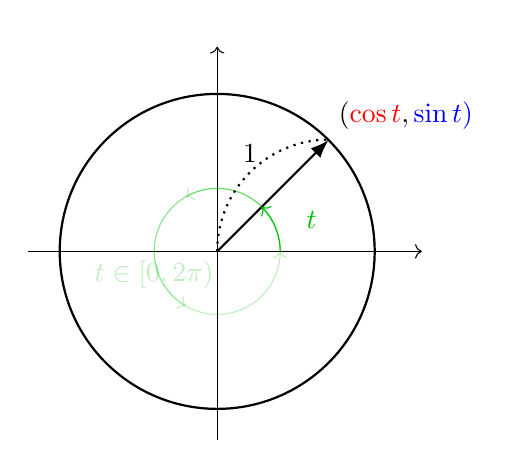
\begin{tikzpicture}[scale=2]
	% Unit circle
	\draw[thick] (0,0) circle(1);
	\draw[->] (-1.2,0) -- (1.3,0) node[right] {};
	\draw[->] (0,-1.2) -- (0,1.3) node[above] {};
	
	% Point at angle t
	\def\t{45}
	\draw[-Latex, thick] (0,0) -- ({cos(\t)}, {sin(\t)}) node[above right] {\(({\color{red}\cos t}, \color{blue}\sin t)\)};
	\draw[->, green!75!black, opacity=.25] (0.4,0) arc[start angle=0, end angle=120, radius=0.4] node[midway, below] {};
	\draw[->, green!75!black, opacity=.25] (0.4,0) arc[start angle=0, end angle=240, radius=0.4] node[midway, below] {};
	\draw[->, green!75!black, opacity=.25] (0.4,0) arc[start angle=0, end angle=360, radius=0.4] node[midway, below] {$t\in\intco{0,2\pi}$};
	\draw[->, green!75!black] (0.4,0) arc[start angle=0, end angle=\t, radius=0.4];
	\node[green!75!black] at (0.6,0.2) {\(t\)};
	% Curve labels
	%\node at (0,-1.5) {\textbf{Figure 1.} Trigonometric parametrization of the unit circle};
	
	\draw[-, dotted, thick] (0,0) arc[start angle=180, end angle=90, radius=.71] node[midway, above] {$1$};
\end{tikzpicture}
\end{minipage}\hfill
\begin{minipage}{.49\textwidth}\centering
	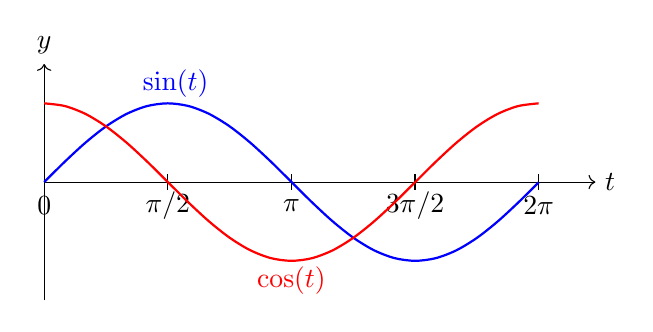
\begin{tikzpicture}[scale=1]
	% Draw axes
	\draw[->] (0,-1.5) -- (0,1.5) node[above] {\(y\)};
	\draw[->] (0,0) -- (7,0) node[right] {\(t\)};
	
	% Mark key points on the t-axis (0, pi/2, pi, 3pi/2, 2pi)
	\foreach \x in {0,1.57,3.14,4.71,6.28} {
		\draw (\x,0.1) -- (\x,-0.1);
	}
	\node at (0,-0.3) {\(0\)};
	\node at (1.57,-0.3) {\(\pi/2\)};
	\node at (3.14,-0.3) {\(\pi\)};
	\node at (4.71,-0.3) {\(3\pi/2\)};
	\node at (6.28,-0.3) {\(2\pi\)};
	
	% Draw sin(t) in blue
	\draw[domain=0:6.28, smooth, variable=\t, blue, thick] 
	plot ({\t},{sin(\t r)});
	\node[blue] at (1.67,1.25) {\(\sin(t)\)};
	
	% Draw cos(t) in red
	\draw[domain=0:6.28, smooth, variable=\t, red, thick] 
	plot ({\t},{cos(\t r)});
	\node[red] at (3.14,-1.25) {\(\cos(t)\)};
\end{tikzpicture}
\end{minipage}
\end{center}
The standard parametrization of \(\mathbb{S}^1\) is given by \[
t \mapsto (\cos t, \sin t), \quad t \in [0,2\pi),
\]
which in turn implies the fundamental trigonometric identity $\cos^2 t + \sin^2 t = 1$. The mapping \[
\fullfunction{\varphi}{\intco{0,2\pi}}{\mathbb{S}^1}{t}{(\cos t,\sin t)}.
\] provides a bijection between the half-open interval \(\intco{0,2\pi}\) and the unit circle $\mathbb{S}^1$.\par Geometrically, it represents the set of points at a fixed distance \(1\) from the origin in \(\mathbb{R}^2\), while algebraically it can be seen as a group under complex multiplication.
\begin{center}
	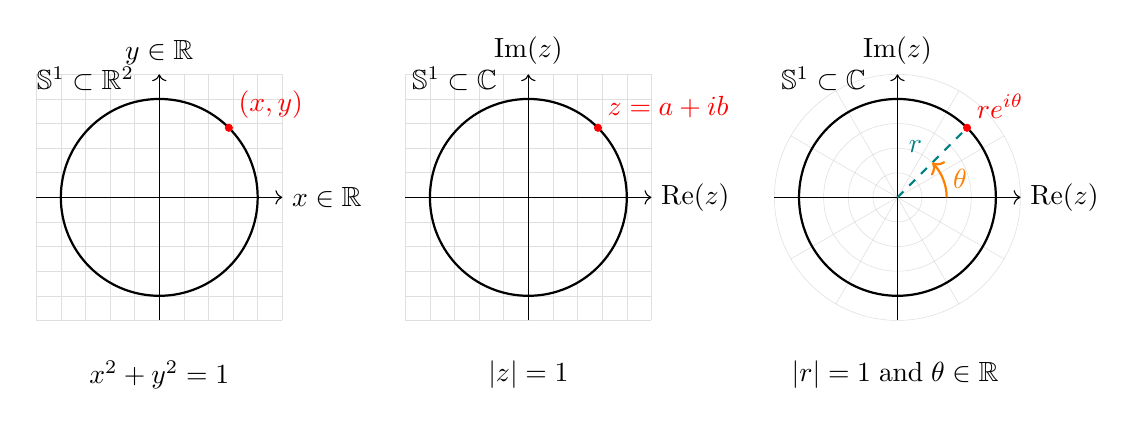
\begin{tikzpicture}[scale=1.25]
		% Left illustration: R^2 representation of the unit circle
		\begin{scope}[xshift=0cm]
			\draw[step=.25cm,gray!50,very thin,opacity=.5] (-1.25,-1.25) grid (1.25,1.25);
			% Axes for R^2
			\draw[->] (-1.25,0) -- (1.25,0) node[right] {$x\in\R$};
			\draw[->] (0,-1.25) -- (0,1.25) node[above] {$y\in\R$};
			% The unit circle in R^2
			\draw[thick] (0,0) circle (1cm);
			% Label the circle with its equation
			\node at (0,-1.8) {\(x^2 + y^2 = 1\)};
			\node at (-.75,1.2) {\(\mathbb{S}^1 \subset \mathbb{R}^2\)};
			\filldraw[red] (45:1cm) circle (1pt) node[above right] {\((x,y)\)};
		\end{scope}
		% Right illustration: Complex plane representation of the unit circle
		\begin{scope}[xshift=3.75cm]
			\draw[step=.25cm,gray!50,very thin,opacity=.5] (-1.25,-1.25) grid (1.25,1.25);
			% Axes for the complex plane
			\draw[->] (-1.25,0) -- (1.25,0) node[right] {\(\Re(z)\)};
			\draw[->] (0,-1.25) -- (0,1.25) node[above] {\(\Im(z)\)};
			% The unit circle in the complex plane
			\draw[thick] (0,0) circle (1cm);
			% Draw an arc to indicate the angle theta
			%		\draw[->, red] (0.5,0) arc (0:45:0.5);
			%		\node at (0.7,0.2) {\(\theta\)};
			% Mark and label a point on the circle corresponding to e^(i theta)
			\filldraw[red] (45:1cm) circle (1pt) node[above right] {\(z = a + ib\)};
			% Label the circle with its modulus condition
			\node at (0,-1.8) {\(|z| = 1\)};
			\node at (-.75,1.2) {\(\mathbb{S}^1 \subset \mathbb{C}\)};
			
			%		\filldraw[red] (1,1) circle (1.5pt) node[anchor=south west, black] {$$};
		\end{scope}
		\begin{scope}[xshift=7.5cm]
			% Draw concentric circles for radii 1 to 5
			\foreach \r in {.25,.5,...,1.25} {
				\draw[very thin, gray!50, opacity=.5] (0,0) circle (\r);
			}
			% Draw radial lines at every 30 degrees
			\foreach \angle in {0,30,...,360} {
				\draw[very thin, gray!50, opacity=.5] (0,0) -- (\angle:1.25);
			}
			
			% Axes for the complex plane
			\draw[->] (-1.25,0) -- (1.25,0) node[right] {\(\Re(z)\)};
			\draw[->] (0,-1.25) -- (0,1.25) node[above] {\(\Im(z)\)};
			% The unit circle in the complex plane
			\draw[thick] (0,0) circle (1cm);
			% Draw an arc to indicate the angle theta
			%		\draw[->, red] (0.5,0) arc (0:45:0.5);
			%		\node at (0.7,0.2) {\(\theta\)};
			% Mark and label a point on the circle corresponding to e^(i theta)
			\filldraw[red] (45:1cm) circle (1pt) node[above right] {\(re^{i\theta}\)};
			% Label the circle with its modulus condition
			\node at (0,-1.8) {\(\abs{r}=1\;\text{and}\;\theta \in \mathbb{R}\)};
			\node at (-.75,1.2) {\(\mathbb{S}^1 \subset \mathbb{C}\)};
			% draw radius
			\draw[dashed, thick, teal] (0,0) -- (.71,0.71) node[midway, above left] {$r$};
			% draw angle
			\draw[->, thick, orange] (0.5,0) arc (0:45:0.5) node[midway, right] {$\theta$};
		\end{scope}
	\end{tikzpicture}
\end{center}
The unit circle can be described in several equivalent ways. In \(\mathbb{R}^2\), it is given by:
\[
\mathbb{S}^1 = \{ (x,y) \in \mathbb{R}^2 : x^2 + y^2 = 1 \}.
\]
In the complex plane, we write:
\[
\mathbb{S}^1 = \{ z \in \mathbb{C} : |z| = 1 \} = \{ re^{i\theta} : \abs{r}=1\;\text{and}\;\theta \in \mathbb{R} \}.
\]
%These representations emphasize the geometric and algebraic property of \(S^1\).
We now show that \(S^1\) forms a group under complex multiplication: \begin{enumerate}[(G1)]
	\item[(G0)] \textbf{(Closure)}\; Let $z_1 = e^{i\theta_1}$ and $z_2 = e^{i\theta_2} \in \mathbb{S}^1.$
	Then $z_1z_2 = e^{i\theta_1}e^{i\theta_2} = e^{i(\theta_1+\theta_2)}\in\mathbb{S}^1.$
	\item \textbf{(Associativity)}\; Let \(z_1=e^{i\theta_1}, z_2=e^{i\theta_2}, z_3=e^{i\theta_3} \in \mathbb{S}^1\) then \[
	(z_1z_2)z_3 = (e^{i\theta_1}e^{i\theta_2})e^{i\theta_3} = e^{i(\theta_1+\theta_2)}e^{i\theta_3} = e^{i(\theta_1+\theta_2+\theta_3)}=e^{i\theta_1}e^{i(\theta_2+\theta_3)}=e^{i\theta_1}(e^{i\theta_2}e^{i\theta_3})= z_1(z_2z_3).
	\]
	\item \textbf{(Identity Element)}\; For each \(z = e^{i\theta} \in S^1\),
	\[
	1 \cdot z = e^{i0}e^{i\theta} = e^{i(0+\theta)}=e^{i\theta} = z,
	\]
	and similarly \(z \cdot 1 = z\).
	\item \textbf{(Inverses)}\; For any \(z = e^{i\theta} \in S^1\), its inverse is given by $
	z^{-1} = e^{-i\theta},$ since
	\[
	z \cdot z^{-1} = e^{i\theta}e^{-i\theta} = e^{i(\theta-\theta)} = e^{i\cdot 0} = 1.
	\]
	Notice that \(e^{-i\theta} \in S^1\) as well.
\end{enumerate}
We show that \textbf{multiplication on the circle group is equivalent to addition of angles}:
let \begin{align*}
	z_1&= r_1e^{i\theta_1}=r_1\of{\cos\theta_1+i\sin\theta_1}\in\C\;\text{and}\\
	z_2&= r_2e^{i\theta_2}=r_2\of{\cos\theta_2+i\sin\theta_2}\in\C.
\end{align*} Then \begin{align*}
	z_1\cdot z_2=r_1e^{i\theta_1}\cdot r_2e^{i\theta_2}=&=r_1r_2\of{\cos\theta_1+i\sin\theta_1}\of{\cos\theta_2+i\sin\theta_2}\\
	&=r_1r_2\left[\of{\cos\theta_1\cos\theta_2-\sin\theta_1\sin\theta_2}+i\of{\cos\theta_1\sin\theta_2+\sin\theta_1\cos\theta_2}\right]\\
	&=r_1r_2\left[\cos\of{\theta_1+\theta_2}+i\sin\of{\theta_1+\theta_2}\right]\\
	&=r\of{\cos\theta+\sin\theta}\ \text{with}\ \begin{cases}
		r=r_1r_2\\
		\theta=\theta_1+\theta_2.
	\end{cases}
\end{align*}
\begin{center}
	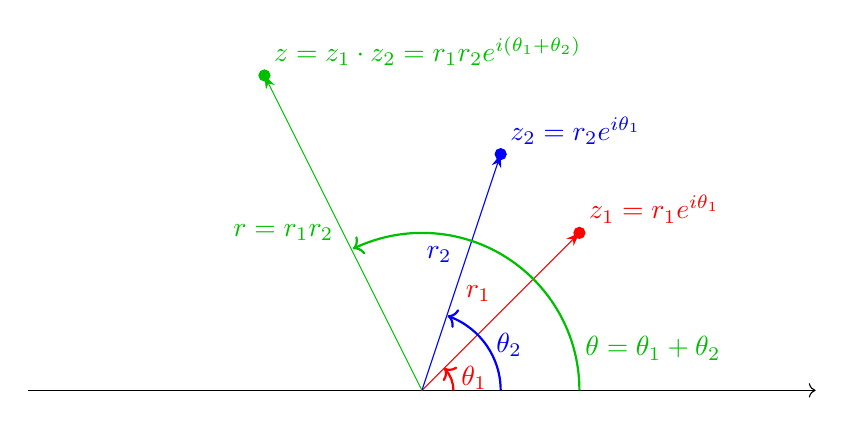
\begin{tikzpicture}[scale=2]
		\draw[->] (-2.5,0) -- (2.5,0) node[right] {};
		\filldraw[red] (1,1) circle (1pt) node[anchor=south west] {$z_1=r_1e^{i\theta_1}$};
		\filldraw[blue] (.5,1.5) circle (1pt) node[anchor=south west] {$z_2=r_2e^{i\theta_1}$};
		\filldraw[green!75!black] (-1,2) circle (1pt) node[anchor=south west] {$z=z_1\cdot z_2=r_1r_2e^{i(\theta_1+\theta_2)}$};
		
		\draw[-Stealth, red] (0,0) -- (1,1) node[midway, above left] {$r_1$};
		\draw[-Stealth, blue] (0,0) -- (.5,1.5) node[midway, above left] {$r_2$};
		\draw[-Stealth, green!75!black] (0,0) -- (-1,2) node[midway, left] {$r=r_1r_2$};
		\draw[->, thick, red] (.2,0) arc (0:45:.2) node[midway, right] {$\theta_1$};
		\draw[->, thick, blue] (.5,0) arc (0:71:.5) node[midway, right] {$\theta_2$};
		\draw[->, thick, green!75!black] (1,0) arc (0:116:1) node[midway, below right=1.25cm] {$\theta=\theta_1+\theta_2$};
	\end{tikzpicture}
\end{center}
\newpage




However, it is important to note that \(S^1\) itself is not a cyclic group because no single element can generate the entire uncountable set. 
A group \(G\) is called \textbf{cyclic} if there exists an element \(g \in G\) such that
\[
G = \langle g \rangle = \{ g^n : n \in \mathbb{Z} \}.
\]
In the context of \(S^1\), while the full group is not cyclic, every finite subgroup of \(S^1\) is cyclic.

\(S^1\) is a compact, connected, and smooth one-dimensional manifold. Its compactness follows from the Heine-Borel theorem, and its connectedness is inherent in the continuity of the circle. These topological features are critical in understanding its role as a topological group.

Though \(S^1\) is a group under multiplication, it is not cyclic. To see this, consider any element \( e^{i\theta} \in S^1 \). The subgroup generated by \( e^{i\theta} \) is:
\[
\langle e^{i\theta} \rangle = \{ e^{in\theta} : n \in \mathbb{Z} \}.
\]
If \(\theta/2\pi\) is irrational, then \(\langle e^{i\theta} \rangle\) is dense in \(S^1\) but does not equal \(S^1\) since it is countable. If \(\theta/2\pi\) is rational, the subgroup is finite. In either case, no single element can generate the entire uncountable group \(S^1\).

The exponential map provides a natural connection between the additive group \(\mathbb{R}\) and the multiplicative group \(S^1\):
\[
\exp: \mathbb{R} \to S^1, \quad \exp(i\theta) = e^{i\theta}.
\]
This continuous group homomorphism is essential in many areas of analysis and differential geometry.
\begin{center}
	\begin{tikzpicture}[>=stealth, scale=0.8]
		% Real line
		\draw[->] (-4,0) -- (4,0) node[right] {\(\mathbb{R}\)};
		\node at (-4,0.3) {\(-\infty\)};
		\node at (4,0.3) {\(+\infty\)};
		
		% S^1: Draw circle to the right
		\begin{scope}[shift={(8,0)}]
			\draw[thick] (0,0) circle (2cm);
			\draw[->] (0,0) -- (2,0) node[right] {$1$};
			\node at (0,2.3) {\(S^1\)};
		\end{scope}
		
		% Arrow from real line to circle (representing the exponential map)
		\draw[->, thick] (2,0.5) -- (7,1.5) node[midway, above] {\(\exp(i\theta)\)};
	\end{tikzpicture}
\end{center}
For any positive integer \(n\), the \(n\)th roots of unity form a finite cyclic subgroup of \(S^1\). Specifically, define:
\[
C_n = \{ e^{2\pi i k/n} : k = 0, 1, \dots, n-1 \}.
\]
This group is cyclic because it can be generated by the element:
\[
e^{2\pi i/n},
\]
and every element in \(C_n\) is a power of this generator.

The cyclic group \(C_n\) is a fundamental object in various fields:
\begin{itemize}
	\item \textbf{Number Theory:} The \(n\)th roots of unity are closely related to cyclotomic polynomials.
	\item \textbf{Signal Processing:} They appear in the discrete Fourier transform (DFT).
	\item \textbf{Algebra:} Finite cyclic groups are among the simplest groups and serve as building blocks for more complex structures.
\end{itemize}

\(S^1\) is not only a topological group but also a Lie group. Its smooth manifold structure enables the study of continuous group representations and provides a gateway into harmonic analysis.

The study of \(S^1\) and its subgroups extends to many areas:
\begin{itemize}
	\item \textbf{Differential Geometry:} \(S^1\) serves as an example of a smooth manifold with a rich geometric structure.
	\item \textbf{Complex Analysis:} As the boundary of the unit disk, \(S^1\) plays a key role in conformal mappings and function theory.
	\item \textbf{Algebraic Topology:} The fundamental group of \(S^1\) is isomorphic to \(\mathbb{Z}\), providing insight into covering spaces and homotopy theory.
\end{itemize}

Recall that a group \(G\) is called \emph{cyclic} if
\[
\exists\, a \in G\;\text{s.t.}\; \forall\, g \in G,\; \exists\, n \in \mathbb{Z}:\; g = a^n.
\]
Consider the circle
\[
S^1 \coloneqq \{\, z \in \mathbb{C} \mid |z|=1 \,\},
\]
which is a group under complex multiplication. Each element of \(S^1\) may be written in the form
\[
z = e^{2\pi i \theta}, \quad \theta \in [0,1),
\]
and for a fixed irrational \(\theta_0\), the subgroup
\[
\langle e^{2\pi i \theta_0} \rangle = \{\, e^{2\pi i n \theta_0} \mid n \in \mathbb{Z} \,\}
\]
is dense in \(S^1\). In the finite setting, for any \(n\in\mathbb{N}\), the subgroup of \(n\)th roots of unity
\[
\mu_n = \{\, e^{2\pi i k/n} \mid k=0,1,\dots,n-1 \,\}
\]
is cyclic, isomorphic to \(\mathbb{Z}/n\mathbb{Z}\).
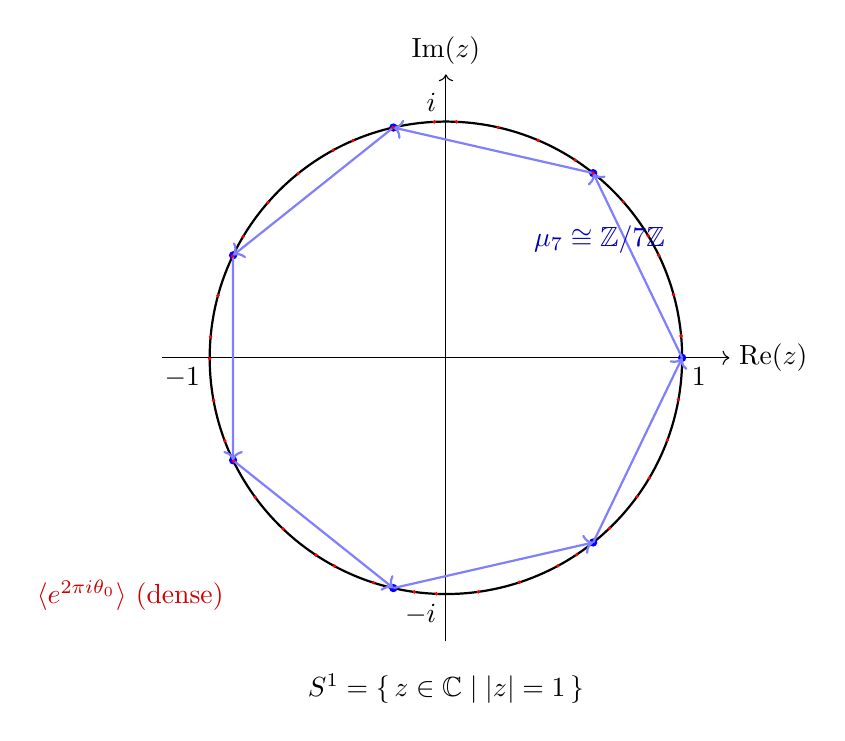
\begin{tikzpicture}[scale=3]
	
	% Draw unit circle and axes
	\draw[thick] (0,0) circle (1);
	\draw[->] (-1.2,0) -- (1.2,0) node[right] {$\Re(z)$};
	\draw[->] (0,-1.2) -- (0,1.2) node[above] {$\Im(z)$};
	
	% Axis labels
	\node[below right] at (1,0) {$1$};
	\node[below left]  at (-1,0) {$-1$};
	\node[above left]  at (0,1) {$i$};
	\node[below left]  at (0,-1) {$-i$};
	
	% Roots of unity: mu_7
	\foreach \k in {0,...,6} {
		\coordinate (mu\k) at ({cos(360/7*\k)},{sin(360/7*\k)});
		\filldraw[blue] (mu\k) circle (0.015);
	}
	
	% Connect cyclically: safer version without 'evaluate'
	\foreach \k in {0,...,6} {
		\pgfmathsetmacro{\next}{mod(\k+1,7)}
		\draw[blue!50, thick, ->] (mu\k) -- (mu\next);
	}
	
	% Label for mu_7
	\node[blue!70!black] at (0.65,0.5) {$\mu_7 \cong \mathbb{Z}/7\mathbb{Z}$};
	
	% Dense subgroup: simulate e^{2\pi i n theta_0} for irrational theta_0
	% Precomputed mod(n*0.4142,1)*360 degrees for n=1..40
	\foreach \angle in {
		149.1, 298.3, 87.4, 236.6, 25.7, 174.9, 324.0,
		113.2, 262.3, 51.5, 200.6, 349.8, 138.9, 288.1,
		77.2, 226.4, 15.5, 164.7, 313.8, 103.0, 252.1,
		41.3, 190.4, 339.6, 128.7, 277.9, 67.0, 216.2,
		5.3, 154.5, 303.6, 92.8, 241.9, 31.1, 180.2,
		329.4, 118.5, 267.7, 56.8, 206.0
	}{
		\fill[red] ({cos(\angle)}, {sin(\angle)}) circle (0.008);
	}
	
	% Labels
	\node[red!80!black, below left] at (-0.9,-0.9) 
	{$\langle e^{2\pi i \theta_0} \rangle$ (dense)};
	\node at (0,-1.4) {$S^1 = \{\, z \in \mathbb{C} \mid |z|=1 \,\}$};
	
\end{tikzpicture}

\newpage
\section{Torus}
\begin{center}
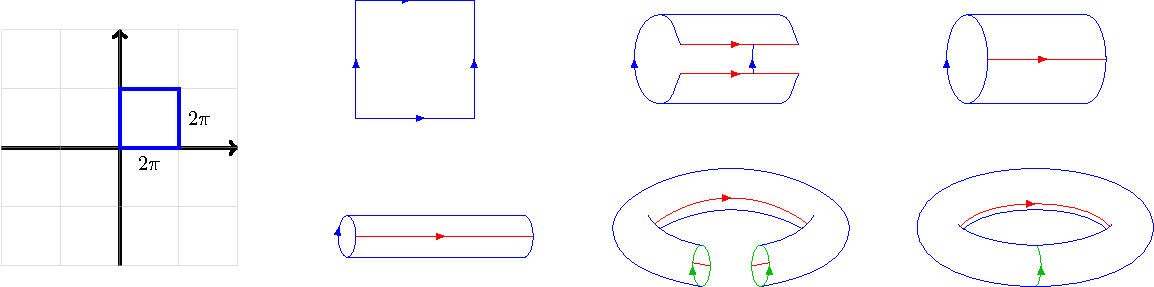
\includegraphics[scale=.85]{../tikz/grad-math-tikz-algebra/torus.pdf}
\end{center}

%\begin{center}
%\tdplotsetmaincoords{70}{110}
%\begin{tikzpicture}[tdplot_main_coords, scale=3]
%	
%	% Define the major and minor radii of the torus
%	\def\R{2} % Major radius (distance from the center of the torus to the center of the tube)
%	\def\r{0.5} % Minor radius (radius of the tube)
%	
%	% Draw curves of constant phi (circles around the tube)
%	\foreach \phi in {0,15,...,345} {
%		\draw[domain=0:360, smooth, variable=\theta, green!75!black, opacity=0.5]
%		plot ({(\R+\r*cos(\theta))*cos(\phi)},{(\R+\r*cos(\theta))*sin(\phi)},{\r*sin(\theta)});
%	}
%	
%	% Draw curves of constant theta (circles along the torus body)
%	\foreach \theta in {0,15,...,345} {
%		\draw[domain=0:360, smooth, variable=\phi, red, opacity=0.5]
%		plot ({(\R+\r*cos(\theta))*cos(\phi)},{(\R+\r*cos(\theta))*sin(\phi)},{\r*sin(\theta)});
%	}
%	% Optionally, label the axes
%%	\draw[->] (0,0,0) -- (3,0,0) node[anchor=north east] {\(x\)};
%%	\draw[->] (0,0,0) -- (0,3,0) node[anchor=north west] {\(y\)};
%%	\draw[->] (0,0,0) -- (0,0,2) node[anchor=south] {\(z\)};
%\end{tikzpicture}
%\end{center}

%The torus is defined as
%\[
%T^2 \coloneqq S^1 \times S^1.
%\]
%Since each factor \(S^1\) is a cyclic group (in both its finite and infinite manifestations), the torus inherits a structure where the two “circulating” (cyclic) directions coexist. In particular, the Lie group structure of \(T^2\) is given by the coordinatewise multiplication:
%\[
%(z_1, w_1) \cdot (z_2, w_2) = (z_1 z_2,\, w_1 w_2).
%\]
%Moreover, its fundamental group is
%\[
%\pi_1(T^2) \cong \pi_1(S^1) \times \pi_1(S^1) \cong \mathbb{Z} \times \mathbb{Z},
%\]
%which is not cyclic but contains many cyclic subgroups (e.g., the subgroup generated by \((p,q)\) with \(\gcd(p,q)=1\)).
%
%Thus, when learning about cyclic groups, one simultaneously gains insight into the structure of the torus: each factor of \(T^2\) embodies the essence of cyclicity, and the torus itself is a geometric object built from these circulating (cyclic) components.
%
%
%
%- **Learning \(S^1\):** One studies the cyclic nature of \(S^1\) through its generators (e.g., \(e^{2\pi i \theta}\)) and observes both finite (roots of unity) and infinite (dense subgroup) cyclic behaviors.
%
%
%- **Understanding \(T^2\):** The torus \(T^2\) is then naturally introduced as the Cartesian product \(S^1 \times S^1\), making the connection explicit: the torus is built from two copies of the cyclic group \(S^1\).
%- **Visualization:** The TikZ diagram visually encapsulates this dual structure, reinforcing that the cyclic groups are the “circulating” components whose product yields the torus.
%
%This integrated approach allows one to simultaneously appreciate the algebraic simplicity of cyclic groups and their geometric realization in the topology of the torus.
%
%\newpage
%Now consider the unit square in the complex plane: from \(0\) to \(1+i\). This forms a fundamental domain for the complex lattice \(\mathbb{Z} + i\mathbb{Z}\), relevant in the study of complex tori and elliptic curves.
%
%\subsection*{Elliptic Curve over \(\mathbb{C}\)}
%
%We now consider the set:
%\[
%E = \left\{ (x,y) \in \mathbb{C}^2 \,\middle|\, y^2 = 4x^3 + 4x \right\}
%\]
%This defines a **complex elliptic curve**, smooth and projective.
%
%\subsection*{Holomorphic Mapping}
%Let \( z \in \mathbb{C} \), and define:
%\[
%z \mapsto (\varphi(z), \varphi'(z))
%\]
%where \( \varphi \) is a suitable elliptic function (e.g., Weierstrass \(\wp(z)\)) satisfying:
%\[
%(\varphi')^2 = 4\varphi^3 + 4\varphi
%\]
%so that the image lies on \( E \).
%
%\begin{center}
%	\begin{tikzpicture}[scale=2.5]
%		
%		% Draw complex plane grid
%		\fill[blue!10,opacity=0.2] (0,0) rectangle (1,1);
%		\draw[step=0.2,gray!50,very thin] (0,0) grid (1.2,1.2);
%		\draw[thick, blue] (0,0) rectangle (1,1);
%		\node at (1.1,1.05) {\(1+i\)};
%		\node at (-0.1,0) {\(0\)};
%		\node at (1.05,0) {\(1\)};
%		\node at (0,1.05) {\(i\)};
%		\node[blue!70!black] at (0.5, -0.2) {\textbf{Fundamental domain in } \(\mathbb{C}\)};
%		
%		% Arrow to curve
%		\draw[->, thick] (1.5,0.5) -- (2.8,0.5) node[midway,above] 
%		{\( z \mapsto (\varphi(z), \varphi'(z)) \)};
%		
%		% Elliptic curve symbolically
%		\begin{scope}[xshift=3.2cm]
%			\draw[domain=-1.2:1.2, smooth, variable=\x, thick, red]
%			plot ({\x}, {\x*\x*\x + \x});
%			\node at (0,-0.5) {\( y^2 = 4x^3 + 4x \)};
%		\end{scope}
%		
%	\end{tikzpicture}
%\end{center}
%\section*{Conclusion}
%
%This sequence of mappings:
%\[
%t \mapsto (\cos t, \sin t) \quad \leadsto \quad z \mapsto (\varphi(z), \varphi'(z))
%\]
%demonstrates a path from elementary trigonometry to deep connections in algebraic and complex geometry — culminating in the geometry of elliptic curves over \(\mathbb{C}\).


\end{document}
